% \begin{figure}[!ht]
% \centering
% 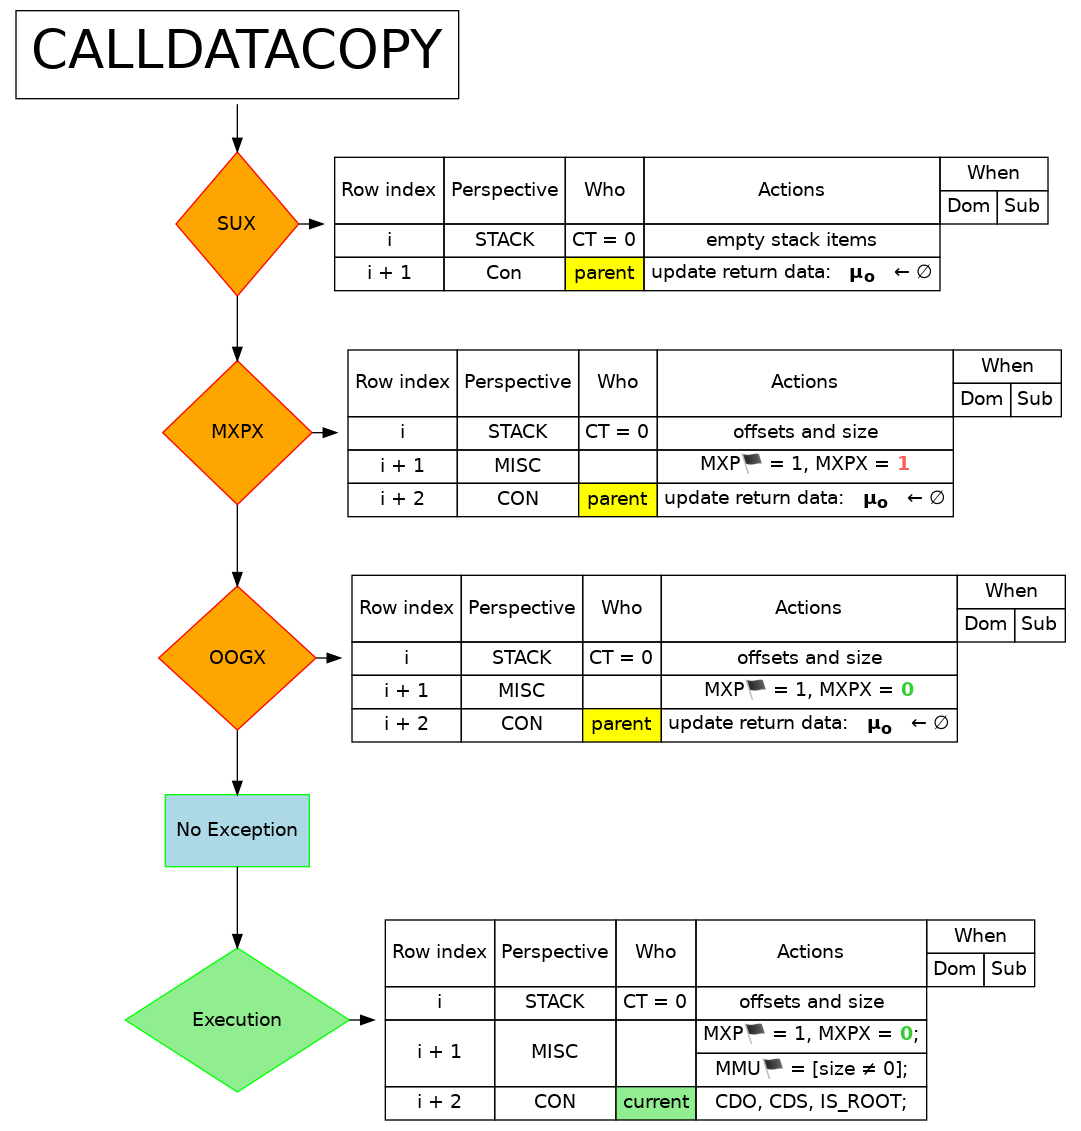
\includegraphics[width=\textwidth]{instruction_handling/copy/flowcharts/cdc.png}
% 	\caption{General workflow for \inst{CALLDATACOPY}-type instructions.}
% \label{hub: call: fig: general processing}
% \end{figure}

\begin{center}
	\boxed{%
		\text{The stack constraints presented below assume }
		\left\{ \begin{array}{lcl}
			\peekStack        _{i}                  & = & 1 \\
			\stackDecCopyFlag _{i}                  & = & 1 \\
			\locIsCdc                               & = & 1 \\
			\stackSux         _{i} + \stackSox _{i} & = & 0 \\
		\end{array} \right.}
\end{center}
In other words we are dealing with a \inst{CALLDATACOPY} instruction that doesn't raise a \suxSH{}.
The specialized constraints are as follows:
\begin{description}
		% - [x] context stuff,
		% - [x] gas cost stuff,
		% - [∅] account stuff,
		% - [∅] trimming stuff,
		% - [∅] setting and unsetting warmth,
		% - [∅] account remain unchanged otherwise,
		% - [∅] etc ...
	\item[\underline{\underline{Setting the gas cost:}}]
		we only set the gas cost to the actual gas cost if no \mxpxSH{} has occurred (given no stack exception, that is):
		\begin{enumerate}
			\item \If $\stackMxpx _{i} = 1$ \Then $\gasCost_{i} = 0$
			\item \If $\stackOogx _{i} = 1$ \Then $\gasCost_{i} = \stackStaticGas_{i} + \locMxpGas$
			\item \If $\xAhoy     _{i} = 0$ \Then $\gasCost_{i} = \stackStaticGas_{i} + \locMxpGas$
		\end{enumerate}
		\saNote{} The above \emph{could} be subsumed under the single constraint
		\[
			\gasCost _{i} = (\stackOogx _{i} + (1 - \xAhoy _{i})) \cdot (\stackStaticGas_{i} + \locMxpGas) \quad (\trash)
		\]
	\item[\underline{\underline{Setting the context-row $n^°(i + \locCopyCurrentContextRow)$:}}]
		depending on whether the instruction produces an exception or not we either peek into the caller context (and provide it with empty return data) or inspect the current execution frame; we extract from it the following: call data offset, call data size and the datum of whether or not it is the root context; as such we impose
		\begin{enumerate}
			\item \If $\xAhoy _{i} = 1$ \Then $\executionProvidesEmptyReturnData {i}{\locCopyCallerContextRowSmall} $ (\trash)
			\item \If $\xAhoy _{i} = 0$ \Then $\readContextData                  {i}{\locCopyCurrentContextRow}{\cn_{i}} $
		\end{enumerate}
\end{description}
